\documentclass{beamer}
\usepackage[utf8]{inputenc}
\usepackage{tikz}
\usepackage{verbatim}
\usepackage{graphicx}
\usetheme{Darmstadt}
\title{ZeroMQ in the Browser}
\author{Ondřej Kupka}

\begin{document}

\begin{frame}
\titlepage
\end{frame}

\section{The Goal}
\begin{frame}{The Goal}
  Initial movings:
  \begin{enumerate}
    \item I like ZeroMQ (0MQ). It's fun to use.\\Service-oriented architecture FTW.
	\item Browser single-page apps are modern...\\And we have Habanero yay!
  \end{enumerate}
  After heavy thinking:
  \begin{itemize}
    \item Let's get 0MQ-based services into the browser!
  \end{itemize}
  And thus the goal appeared to be:
  \begin{itemize}
    \item A super cool library to somehow manage 0MQ services from the browser,
	      as much as cool you can be with JavaScript.
	\item Make it easy to implement all the well-known 0MQ patters
	      (Lazy Pirate, Majordomo, \ldots)
  \end{itemize}
\end{frame}

\section{Initial Research}
\subsection{Available Solutions}
\begin{frame}{Initial Research - NullMQ}
  What ideas are behind NullMQ?
  \begin{enumerate}
    \item More or less imitate 0MQ sockets in the browser.\\
	      In a sucky way, though\ldots
	\item Tunnel it to the server using STOMP.
	\item From there use the real 0MQ to get to the services.
  \end{enumerate}
  What I found out after studying this was that to tunnel
  0MQ sockets and imitate them in the browser is probably not a good
  approach. It's a PITA to implement all the complex 0MQ patterns
  there. More like impossible...
  \\~\\
  Conclusion: Move the complex part to the server.
\end{frame}

\begin{frame}{Initial Research - SocketMQ}
  This is a very new attempt to bring 0MQ-like semantics into the browser.
  Not very successful for now. Doesn't look like it will ever be.
  \\~\\
  Conclusion: The library sucks for now, but I could also use socket.io
  as they do, or something similar. Well, in the end it will be probably SockJS.
\end{frame}

\begin{frame}{Initial Research - API Clients the 0MQ Way}
  \begin{center}
	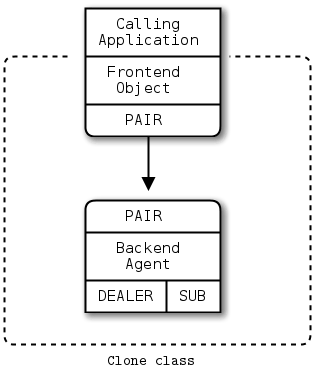
\includegraphics[width=\textwidth,height=0.8\textheight,keepaspectratio]{Resources/multithreading-api.png}
  \end{center}
\end{frame}

\subsection{Conclusion}
\begin{frame}{Initial Research - Conclusion}
  So what to do basically:
  \begin{enumerate}
    \item Client frontend is a proxy object living in the browser,
	      sending commands to the backend part living on the server.
	\item Use SockJS to imitate 0MQ point-to-point PAIR socket connection.
  \end{enumerate}
  Advantages:
  \begin{itemize}
    \item Simple calls to the proxy object in the browser.
	\item Complex communication on the server side is easier to implement.
  \end{itemize}
  Disadvantages:
  \begin{itemize}
    \item 0MQ PAIR != (!==) SockJS Internet-scale connection. It can break,
	      you have to manage SockJS connection, multiplex them and stuff.
  \end{itemize}
\end{frame}

\section{State of the Affairs}
\begin{frame}{State of Affairs - The Browser API}
  Didn't know that it's so difficult to come up with a solid library API...
  \begin{center}
	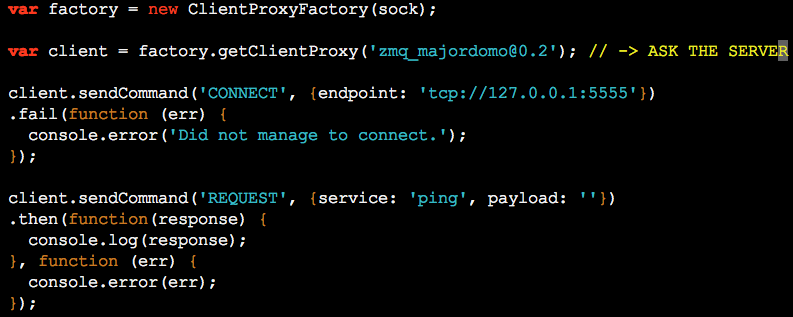
\includegraphics[width=\textwidth,height=0.9\textheight,keepaspectratio]{Resources/browser-api.png}
  \end{center}
  No, don't worry, that was not the solid one yet!
\end{frame}

\begin{frame}{State of the Affairs - The Server API}
  Not really sure about the internals yet, but this is how a client should
  be done. More or less.
  \begin{center}
	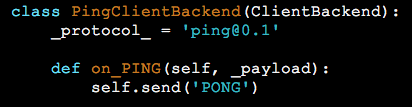
\includegraphics[width=\textwidth,height=0.9\textheight,keepaspectratio]{Resources/server-api.png}
  \end{center}
  Then you only add it to the router and it detends and assigns the protocol
  automatically. Pretty easy!
\end{frame}

\begin{frame}{State of the Affairs - Summary}
  Got to the point when I started asking myself again:\\Someone else must have
  done the same thing before, right?\\Well, I haven't managed to find it... for now.
  \\If you manage before me, please stop me before I implement it myself! Thank you.
  \\~\\
  Anyway, any questions?
  \\~\\
  Thanks!
\end{frame}
\end{document}
